\chapter{序論}

\section{研究背景}

移動ロボットが自己位置を推定する方法として確率的な位置推定法である
パーティクルフィルターがよく用いられる. 
用いられている例として, rosのナビゲーションスタックである
amcl\cite{amcl_github}や千葉工業大学未来ロボティクス学科の上田隆一准教授が
開発したemcl\cite{emcl_github}がある. 
%%%%開発者って私じゃなくて?
パーティクルフィルターは現在の状態から推定される次のロボットの
状態の候補として多数のパーティクルに置き換え, 
%%%%ちょっと文がおかしい. パーティクルを次のロボットの状態の候補と見立てるんじゃなくて?「見立てる」は別の動詞に変えたほうがいいかも. 
予測と観測によりパーティクルの更新を行うことで自己位置を推定するアルゴリズムである. 
%%%%重みつき平均じゃなくて最尤なパーティクルの場合もあるのでこれはダウト. もうちょっと大雑把にせつめいしたほうがよい. 

安定的に自己位置推定を行うことは, 移動ロボットが
ある目標へと自律移動を行うために重要である. 
パーティクルフィルターにおいて何らかの理由で
全パーティクルの尤もらしさが低い場合, 
自己位置推定を誤ってしまう. 
%%%%この時点で尤度とかあんまり使わないほうがいいと思う. もっと誰にでも分かる表現はないでしょうか?
%%%%「見失う」というのは口語です. 別の言葉に. 
自己位置推定を誤ったまま行動をし続けてしまった場合, 
ロボットが走行できない状態になってしまう. 
%%%%↑もっと話を膨らます. だとしたらどんな困ったことがあるのか. そして, どうなればよくなるのか. 
そのような例として, 以下のような例がある. 

\begin{itemize}
  \item 観測できない低い障害物と衝突し, スタック
  \item 経路計画が不安定になり, スタック
  \item 誘拐問題\cite{gutmann2002etal}に発展し, スタック
\end{itemize}

自己位置推定を誤ってしまう原因として未知障害物の観測がある. 
未知障害物は図\ref{fig:unknown-obstacles}, \ref{fig:known-obstacles}
のような既知のマップに含まれていない観測情報のことである. 
例えば, 既知のマップに対して未知障害物である車や人を含んだ観測情報
をパーティクルの尤度計算に用いた場合, 全パーティクルの尤もらしさが低下する. 
また, 未知障害物への対策を講じていなければ, 未知障害物が観測情報に含まれている間は
常に全パーティクルの尤もらしさが低下し続け, パーティクルの分布は大きく広がってしまい, 
自己位置推定が破綻してしまう. また, 自己位置推定を誤ってしまった状態に対しての回復策として
様々なリセット法がある. 
例えば, amclは前回より尤度平均が小さくなるとランダムパーティクルを注入する. 
emclは尤度平均がある任意の閾値より小さくなった場合, 
任意の範囲内にパーティクルを配置をする\cite{ueda2004iros}. 
それぞれのリセットはいずれも尤度がある値を下回った時にかかり, 
パーティクルの分布を真値周辺に近づけることができる. 
しかし, 効果的なリセットではあるが未知障害物を観測した場合, 
不要なリセットが何度もかかってしまうことで, かえって自己位置推定に悪影響を与える
ことがある. 
このような場合, 全てのパーティクルにおいて, 何らかの方法により
未知障害物を含まない同じ観測情報を使用するような, 
未知障害物を含んだ観測情報を尤度計算に使用しないことによる解決方法が考えられる. 
そのため, 本稿ではパーティクルが未知障害物を含まない観測情報を使用する方法について着目した. 

\begin{figure}[htbp]
  \begin{minipage}[b]{0.5\linewidth}
    \centering
    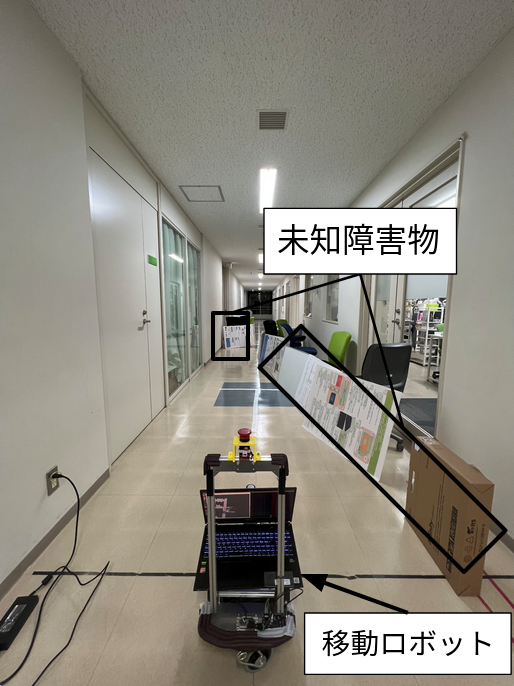
\includegraphics[keepaspectratio, scale=0.32]{figs/unknown_obstacles.png}
    \caption{未知障害物を含んだ屋内環境}
    \label{fig:unknown-obstacles}
  \end{minipage}
  \begin{minipage}[b]{0.5\linewidth}
    \centering
    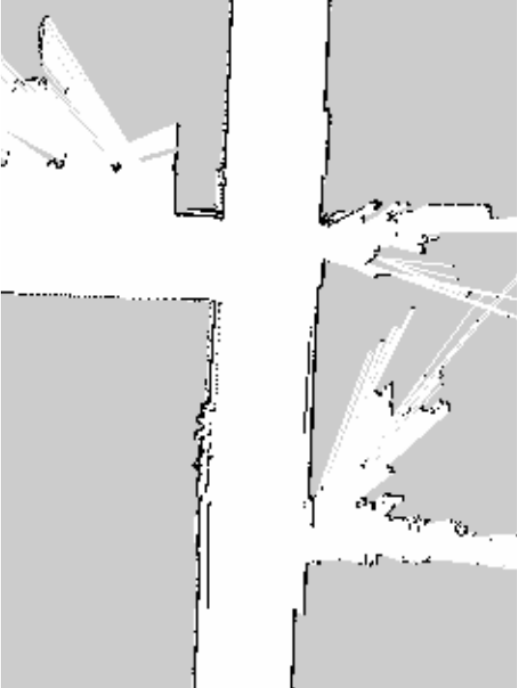
\includegraphics[keepaspectratio, scale=0.32]{figs/known_obstacles.png}
    \caption{未知障害物を含んでいない地図}
    \label{fig:known-obstacles}
  \end{minipage}
\end{figure}

%%%%ここで段落は分ける. というか, 1.2: 従来研究に移行しましょう. これ以降はまた次の機会に見ます. 
%%%%掛かる<-漢字の間違い

\section{従来研究}

安定的に自己位置推定を行うためには未知障害物に対応するアルゴリズムが必要である.
そのため, 自己位置推定において未知障害物に対応するための研究事例\cite{富沢2012}\cite{赤井2019}がある. 
\cite{富沢2012}はセンサの観測情報から得られたローカル地図と既知の地図
とで重なり合ったピクセルごとの差異を求め不一致のピクセル数から
そのパーティクルの尤もらしさを判定する方法による未知障害物の対策を提案している. 
この方法の場合, 使用するセンサの計測距離に応じてマッチングに使用するための地図が大きくなり、
ピクセルごとの差異を求める際の計算コストの増加が考えられる. 
また, \cite{赤井2019}はロボットの位置と地図上での観測物体の有無を同時に推定することで存在する障害物か
ら得られている観測情報のみを有効利用する未知障害物の対策を提案している. 
この方法は尤度場モデルを使用したパーティクルフィルタより, わずかであるが計算時間が増加してしまっている. 
また, 未知障害物を含まないセンサ情報を使用する場合, 過度に観測情報を間引いてしまうことによる
自己位置推定の破綻が考えられる. 

そこで本稿では各パーティクルごとにある決められた観測範囲を尤度計算に用いることで
計算時間の増加が伴わない単純なアルゴリズムで未知障害物に対応する方法を提案する. 
未知障害物が含まれていない観測範囲が与えられたパーティクルであれば, 
そのパーティクルの尤もらしさは高くなる. 
各パーティクルが持つ観測情報は, 尤度計算を繰り返し行うことで最適な観測範囲が収束し, 求められる. 
また、決められた観測範囲を与えることによって、過度に観測情報を間引くことなく、ロバストな自己位置推定を
行える。

\section{研究目的}
以上の議論から、本研究は\\
各パーティクルごとにある決められた観測範囲を尤度計算に用いることにより、
従来の尤度場モデルを使用した自己位置推定と比べて、計算時間の増加無しに
未知障害物に対応するアルゴリズムの開発\\
を目的とする。

また、以下の項目を達成することを目標とし、開発したアルゴリズムを用いた実験を行う。

\begin{enumerate}
  \item 未知障害物による極端な尤度の低下を防ぎ、安定的な自己位置推定を行う
  \item 未知障害物に対して最適な観測範囲を求め、自己位置推定の不要なリセットを防ぐ
\end{enumerate}

\section{本論文の構成}
% この方法については@@@章で話す. 
